\documentclass{article}\usepackage[]{graphicx}\usepackage[]{color}
%% maxwidth is the original width if it is less than linewidth
%% otherwise use linewidth (to make sure the graphics do not exceed the margin)
\makeatletter
\def\maxwidth{ %
  \ifdim\Gin@nat@width>\linewidth
    \linewidth
  \else
    \Gin@nat@width
  \fi
}
\makeatother

\definecolor{fgcolor}{rgb}{0.345, 0.345, 0.345}
\newcommand{\hlnum}[1]{\textcolor[rgb]{0.686,0.059,0.569}{#1}}%
\newcommand{\hlstr}[1]{\textcolor[rgb]{0.192,0.494,0.8}{#1}}%
\newcommand{\hlcom}[1]{\textcolor[rgb]{0.678,0.584,0.686}{\textit{#1}}}%
\newcommand{\hlopt}[1]{\textcolor[rgb]{0,0,0}{#1}}%
\newcommand{\hlstd}[1]{\textcolor[rgb]{0.345,0.345,0.345}{#1}}%
\newcommand{\hlkwa}[1]{\textcolor[rgb]{0.161,0.373,0.58}{\textbf{#1}}}%
\newcommand{\hlkwb}[1]{\textcolor[rgb]{0.69,0.353,0.396}{#1}}%
\newcommand{\hlkwc}[1]{\textcolor[rgb]{0.333,0.667,0.333}{#1}}%
\newcommand{\hlkwd}[1]{\textcolor[rgb]{0.737,0.353,0.396}{\textbf{#1}}}%
\let\hlipl\hlkwb

\usepackage{framed}
\makeatletter
\newenvironment{kframe}{%
 \def\at@end@of@kframe{}%
 \ifinner\ifhmode%
  \def\at@end@of@kframe{\end{minipage}}%
  \begin{minipage}{\columnwidth}%
 \fi\fi%
 \def\FrameCommand##1{\hskip\@totalleftmargin \hskip-\fboxsep
 \colorbox{shadecolor}{##1}\hskip-\fboxsep
     % There is no \\@totalrightmargin, so:
     \hskip-\linewidth \hskip-\@totalleftmargin \hskip\columnwidth}%
 \MakeFramed {\advance\hsize-\width
   \@totalleftmargin\z@ \linewidth\hsize
   \@setminipage}}%
 {\par\unskip\endMakeFramed%
 \at@end@of@kframe}
\makeatother

\definecolor{shadecolor}{rgb}{.97, .97, .97}
\definecolor{messagecolor}{rgb}{0, 0, 0}
\definecolor{warningcolor}{rgb}{1, 0, 1}
\definecolor{errorcolor}{rgb}{1, 0, 0}
\newenvironment{knitrout}{}{} % an empty environment to be redefined in TeX

\usepackage{alltt}
\usepackage{amssymb}
\usepackage{enumerate}
\usepackage{relsize}
\usepackage{url} % not crucial - just used below for the URL
\usepackage{multirow}
\usepackage{multicol}
\usepackage{rotating}
\usepackage{relsize}
\usepackage{bm}
\usepackage{framed}
%\usepackage{empheq}
\usepackage{hyperref}
\usepackage{multicol}
\usepackage{setspace}
\usepackage{enumerate}
\usepackage{footnote}
\usepackage{authblk}
\usepackage{float}
\usepackage{longtable}
\def\a{\alpha}      \def\b{\beta}     \def\g{\gamma}   \def\d{\delta}
\def\th{\theta}     \def\lm{\lambda}  \def\sg{\sigma}
\def\lmone{\lambda_{1n}}
 \def\lmtwo{\lambda_{2n}}
\def\bzero{{\mathbf 0}}  \def\bone{{\mathbf 1}} \def\btwo{{\mathbf 2}}
\def\bW{{\mathbf W}}
\def\bB{{\mathbf B}}
\def\bA{{\mathbf A}} \def\bC{{\mathbf C}} \def\bD{{\mathbf D}} \def\bE{{\mathbf E}}
\def\bF{{\mathbf F}} \def\bS{{\mathbf S}} \def\bT{{\mathbf T}}
\def\bG{{\mathbf G}} \def\bH{{\mathbf H}} \def\bK{{\mathbf K}} \def\bI{{\mathbf I}}
\def\bL{{\mathbf L}} \def\bN{{\mathbf N}} \def\bP{{\mathbf P}} \def\bQ{{\mathbf Q}}
\def\bR{{\mathbf R}} \def\bS{{\mathbf S}} \def\bT{{\mathbf T}} \def\bU{{\mathbf U}}
\def\bV{{\mathbf V}} \def\bW{{\mathbf W}} \def\bX{{\mathbf X}} \def\bY{{\mathbf Y}}
\def\bZ{{\mathbf Z}}
\def\bM{\boldsymbol M}
\def\bPi{{\mathbf \Pi}}

\def\tbM{\widetilde{\boldsymbol M}}
\def\tT{\widetilde{T}}

\def\ba{{\mathbf a}} \def\bb{{\mathbf \beta}}
\def\bd{{\mathbf d}} \def\be{{\mathbf e}}
\def\bdf{{\mathbf f}} \def\bg{{\mathbf g}} \def\bh{{\mathbf h}}

\def\bell{{\mathbf l}} \def\bp{{\mathbf p}} \def\bq{{\mathbf q}}
\def\br{{\mathbf r}} \def\bs{{\mathbf s}} \def\bt{{\mathbf t}}
\def\bu{{\mathbf u}} \def\bv{{\mathbf v}} \def\bw{{\mathbf w}}
\def\bx{{\mathbf x}} \def\by{{\mathbf y}} \def\bz{{\mathbf z}}
\def\bSigma{{\mathbf \Sigma}}
%\newcommand{\bm}{\mathbf}
\newcommand{\argmin}[2]{\underset{#1}{\arg\min} \{ #2\}}
\newcommand{\Argmin}[2]{\underset{#1}{\arg\min} \Bigg \{ #2 \Bigg \} }
\newcommand{\RR}{\mathbb{R}}

%% new
 \def\bbeta{{\mathbf \beta}}
 \def \tbbeta{{ \tilde{\mathbf \beta}}}
 \def \tbw{{\tilde{\bw}}}
 \def \cR{{\cal {R}}}
 \def \hbw{{\hat{\bw}}}
 \def \hbbeta{\mathbf {\hat{\beta}} }
 \def \hbeta{\hat{\b}}
 \def \hw{{\hat{w}}}
 \def \hb{{\hat{\b}}}
 \def \eps{ \epsilon}
 \def \btheta{\mathbf \theta}
 \def \bPsi{\mathbf \Psi }
 \def \bOmega { \mathbf \omega}
 \def \veps{\epsilon}
 \def \bveps{ \mathbf \epsilon}
 \def \cA{ \mathbb{A}} % dont know what it is \mathbb{text}
 \def \beps {\mathbf \epsilon }
\def \tbnu{ \tilde{\mathbf{\nu}}}
\def \tnu { \tilde{\nu}}
\def \hbtheta { \hat{\mathbf \theta}}
\def \bpsi {\mathbf \psi }
\def \bTheta { \mathbf \Theta}
\def \rm { }
\def \tbW { \tilde{\mathbf W}}
\def \bnu { \mathbf \nu}
\def \hbSigma {  \hat{ \mathbf \Sigma}}
\def \diag {diag}
\IfFileExists{upquote.sty}{\usepackage{upquote}}{}
\begin{document}
\section{Numerical Result}



% ----------------------------- Variable Selection for Low dimensional case ------------------------------------%
\begin{table}[thp]
	\begin{center}
	 \caption{Variable Selection Results for Example 1 ($\bbeta=(3,2,1.5,0,0,0,0,0)'$ with 10\% outliers ) }\label{table-selection-low1}
	\begin{tabular}{ccccccccccc}\\\hline\hline
	    Method  & CFR (\%) & OFR (\%) & AN & TIME & & & CFR (\%) & OFR (\%) & AN & TIME\\ \hline
	
	   & \multicolumn{4}{c} {\bf Case A} & && \multicolumn{4}{c} {\bf Case B}  \\
	   
	    ALasso & 74 & 23 & 3.29  & 0.8
	         &&& 63 & 25 & 3.25 & 0.78\\
	    
	    sLTS & 9 & 89 & 6.19  &  358.85
	         &&& 14 & 86 & 5.92 &  357.24\\
	    
	    MMNNG & 68 & 25 & 3.25  &  691.33
	    &&& 88 & 12 & 3.13 &  682.07\\
	    
	    SROS & 21 & 76 & 4.31 &  56.67 & && 31 & 69 & 4.24 & 51.79 \\
	         
	    %PAWLS(0) & 58 & 41 & 3.51  &  && 61 & 39 & 3.48 \\
	    
	    PAWLS & 38 & 56 & 3.68 &  16.41 &&& 64 & 36 & 3.42 &  19.32\\
	    APAWLS & 61 & 28 & 3.27 &  20.04 &&& 89 & 11 & 3.11 &  20.18\\
	\\
	   & \multicolumn{4}{c} {\bf Case C} & &  & \multicolumn{4}{c} {\bf Case D}\\
	   
	    ALasso & 3 & 2 & 1.94 & 0.73 &  && 0 & 19 & 2.52 & 0.99\\
	    
	    sLTS & 28 & 72 & 5.34  &  384.69& && 21 & 79 & 5.71 &  398.44\\
	    
	    MMNNG & 72 & 12 & 2.95  &  673.93 &&& 63 & 16 & 3.25  &  682.47\\
	    
	    SROS & 41 & 50 & 3.7  &  50.24 & && 8 & 80 & 4.76  &  50.31\\
	    %PAWLS(0) & 56 & 43 & 3.59 & && 44 & 52 & 4.13 \\
	     PAWLS & 52 & 44 & 3.64  &  21.1& && 98 & 0 & 2.98 &  22.83\\
	    APAWLS & 74 & 20 & 3.19  &  21.78& && 97 & 0 & 2.97 &  23.66\\
	    \\
	    
	     & \multicolumn{4}{c} {\bf Case E} & &  \\
	     ALasso & 5 & 10 & 2.72 & 0.72 &  &\\
	    
	    sLTS & 23 & 77 & 5.7  &  383.1& &\\
	    
	    MMNNG & 73 & 10 & 3.04  &  675.46 &&\\
	    
	     SROS & 26 & 61 & 4.45  &  50.08 & &\\
	    %PAWLS(0) & 56 & 55 & 5.59 & && 55 & 52 & 5.15 \\
	    PAWLS & 55 & 39 & 3.48  &  21.01& &\\
	    APAWLS & 79 & 15 & 3.16  &  22.5& &\\
	    
	        \hline \hline
	\end{tabular}
	\end{center}
	\end{table}
	% 
	% %----------------------------------- 20% outliers ----------------------------------------------------%
	\begin{table}[thp]
	\begin{center}
	 \caption{Variable Selection Results for Example 1 ($\bbeta=(3,2,1.5,0,0,0,0,0)'$ with 20\% outliers ) }\label{table-selection-low2}
	\begin{tabular}{ccccccccccc}\\\hline\hline
	    Method  & CFR (\%) & OFR (\%) & AN & TIME & & & CFR (\%) & OFR (\%) & AN & TIME\\ \hline
	   & \multicolumn{4}{c} {\bf Case C} & &  & \multicolumn{4}{c} {\bf Case D}\\

	    ALasso & 1 & 2 & 1.22 & 0.7 &  && 1 & 4 & 1.68 & 1.19\\

	    sLTS & 25 & 75 & 5.18  &  426.53& && 17 & 82 & 6.1 &  440.39\\

	    MMNNG & 65 & 5 & 2.76  &  470.24 &&& 31 & 33 & 3.96  &  473.42\\

	     SROS & 47 & 45 & 3.62  &  50.14 & && 3 & 75 & 5.15  &  50.54\\
	    %PAWLS(0) & 56 & 43 & 3.59 & && 44 & 52 & 4.13 \\
	    
	    PAWLS & 47 & 49 & 3.65  &  21.51& && 95 & 0 & 2.97 &  24.83\\
	    
	    PAWLS & 78 & 12 & 3.02  &  22.14& && 92 & 0 & 2.94 &  25.29\\
	    \\

	     & \multicolumn{4}{c} {\bf Case E} & &  \\
	     ALasso & 3 & 3 & 1.29 & 0.79 &  &\\

	    sLTS & 27 & 73 & 5.16  &  417.6& &\\

	    MMNNG & 54 & 3 & 3.06  &  688.65 &&\\

	    SROS & 23 & 49 & 4.64  &  51.28 & &\\
	    %PAWLS(0) & 56 & 55 & 5.59 & && 55 & 52 & 5.15 \\
	    PAWLS & 53 & 42 & 3.52  &  21.57& &\\
	    APAWLS & 64 & 10 & 2.86  &  23.87& &\\

	        \hline \hline
	\end{tabular}
	\end{center}
	\end{table}
	% 
	% 	%----------------------------------- 30% outliers ----------------------------------------------------%
	\begin{table}[thp]
	\begin{center}
	 \caption{Variable Selection Results for Example 1 ($\bbeta=(3,2,1.5,0,0,0,0,0)'$ with 30\% outliers ) }\label{table-selection-low3}
	\begin{tabular}{ccccccccccc}\\\hline\hline
	    Method  & CFR (\%) & OFR (\%) & AN & TIME & & & CFR (\%) & OFR (\%) & AN & TIME\\ \hline
	   & \multicolumn{4}{c} {\bf Case C} & &  & \multicolumn{4}{c} {\bf Case D}\\

	    ALasso & 2 & 0 & 0.68 & 0.78 &  && 0 & 3 & 0.96 & 1.34\\

	    sLTS & 1 & 34 & 4.52  &  421.79& && 0 & 95 & 6.84 &  459.78\\

	    MMNNG & 38 & 1 & 2.3  &  465.41 &&& 5 & 41 & 4.29  &  477.06\\

	    SROS & 49 & 38 & 3.5  &  51.07 & && 1 & 76 & 5.17  &  53.23\\
	    %PAWLS(0) & 56 & 43 & 3.59 & && 44 & 52 & 4.13 \\
	    PAWLS & 45 & 47 & 3.5  &  21.54& && 93 & 0 & 2.93 &  26.08\\
	    APAWLS & 77 & 10 & 2.98  &  22.41& && 89 & 0 & 2.89 &  26.66\\
	    \\

	     & \multicolumn{4}{c} {\bf Case E} & &  \\
	     ALasso & 0 & 3 & 1.15 & 0.79 &  &\\

	    sLTS & 0 & 76 & 7.1  &  428.75& &\\

	    MMNNG & 6 & 21 & 3.97  &  704.12 &&\\

	     SROS & 9 & 44 & 5.1  &  52.25 & &\\
	    %PAWLS(0) & 56 & 55 & 5.59 & && 55 & 52 & 5.15 \\
	    PAWLS & 54 & 21 & 3.06  &  21.85& &\\
	    PAWLS & 52 & 4 & 2.57  &  24.28& &\\

	        \hline \hline
	\end{tabular}
	\end{center}
	\end{table}
% ----------------------------- Variable Selection for high dimensional case ------------------------------------%
% ----------------------------- 10% outliers --------------------------------------------------------------------%
\begin{table}[thp]
	\begin{center}
	 \caption{Variable Selection Results for Example 2 ($\bbeta=({\bf 2}_{10}',\bzero_{p-10}')'$ with 10\% outliers  }\label{table-selection-high1}
	\begin{tabular}{ccccccccccc}\\\hline\hline
	    Method  & CFR (\%) & OFR (\%) & AN & TIME & & & CFR (\%) & OFR (\%) & AN & TIME\\ \hline
	
	   & \multicolumn{4}{c} {\bf Case A} & && \multicolumn{4}{c} {\bf Case B}  \\
	   
	    ALasso & 97 & 0 & 9.96  & 3.4
	         &&& 84 & 1 & 9.75 & 3.41\\
	    
	    sLTS & 0 & 84 & 61.38  &  \ensuremath{3.16\times 10^{4}}
	         &&& 0 & 93 & 58.23 &  \ensuremath{3.03\times 10^{4}}\\
	         
	  PAWLS & 6 & 94 & 15.65 &  348.92 &&& 5 & 95 & 14.29 &  356.33\\
	\\
	    APAWLS & 94 & 1 & 9.89 &  399.08 &&& 91 & 0 & 9.5 &  421.68\\
	\\
	   & \multicolumn{4}{c} {\bf Case C} & &  & \multicolumn{4}{c} {\bf Case D}\\
	   
	    ALasso & 0 & 0 & 6.25 & 4.07 &  && 0 & 1 & 6.89 & 4.07\\
	    
	    sLTS & 0 & 95 & 62.58  &  \ensuremath{3.11\times 10^{4}}& && 0 & 96 & 62.73 &  \ensuremath{3.09\times 10^{4}}\\
	   
	   PAWLS & 3 & 96 & 16.12  &  525.96& && 3 & 96 & 16.19 &  492.91\\
	    \\
	    
	    APAWLS & 85 & 0 & 9.84  &  575.21& && 85 & 0 & 9.84 &  541.23\\
	    \\
	    
	     & \multicolumn{4}{c} {\bf Case E} & &  \\
	     ALasso & 0 & 0 & 12.18 & 4.06 &  &\\
	    
	    sLTS & 0 & 97 & 62.63  &  \ensuremath{3.11\times 10^{4}}& &\\
	    
	    PAWLS & 4 & 96 & 16.35  &  524.59& &\\
	    
	    APAWLS & 88 & 0 & 9.88  &  569.03& &\\
	    
	        \hline \hline
	\end{tabular}
	\end{center}
	\end{table}

% ----------------------------- 20% outliers --------------------------------------------------------------------%
\begin{table}[thp]
	\begin{center}
	 \caption{Variable Selection Results for Example 2 ($\bbeta=({\bf 2}_{10}',\bzero_{p-10}')'$ with 20\% outliers  }\label{table-selection-high2}
	\begin{tabular}{ccccccccccc}\\\hline\hline
	    Method  & CFR (\%) & OFR (\%) & AN & TIME & & & CFR (\%) & OFR (\%) & AN & TIME\\ \hline
	   & \multicolumn{4}{c} {\bf Case C} & &  & \multicolumn{4}{c} {\bf Case D}\\
	   
	    ALasso & 0 & 0 & 5.7 & 6.45 &  && 0 & 0 & 6.15 & 6.89\\
	    
	    sLTS & 0 & 69 & 65.89  &  \ensuremath{3.17\times 10^{4}}& && 0 & 96 & 63.61 &  \ensuremath{3.15\times 10^{4}}\\
	    
	    PAWLS & 1 & 98 & 16.67  &  633.1& && 1 & 98 & 17.23 &  588.62\\
	    
	    APAWLS & 79 & 0 & 9.6  &  670.79& && 82 & 0 & 9.73 &  624.28\\
	    \\
	    
	     & \multicolumn{4}{c} {\bf Case E} & &  \\
	     ALasso & 0 & 0 & 17.41 & 6.3 &  &\\
	    
	    sLTS & 0 & 68 & 66.41  &  \ensuremath{3.18\times 10^{4}}& &\\
	    PAWLS & 0 & 99 & 16.89  &  629.49& &\\
	    
	    APAWLS & 78 & 0 & 9.62  &  665.07& &\\
	    
	        \hline \hline
	\end{tabular}
	\end{center}
	\end{table}
	

% ----------------------------- 30% outliers --------------------------------------------------------------------%
\begin{table}[thp]
	\begin{center}
	 \caption{Variable Selection Results for Example 2 ($\bbeta=({\bf 2}_{10}',\bzero_{p-10}')'$ with 30\% outliers  }\label{table-selection-high3}
	\begin{tabular}{ccccccccccc}\\\hline\hline
	    Method  & CFR (\%) & OFR (\%) & AN & TIME & & & CFR (\%) & OFR (\%) & AN & TIME\\ \hline
	   & \multicolumn{4}{c} {\bf Case C} & &  & \multicolumn{4}{c} {\bf Case D}\\
	   
	    ALasso & 0 & 0 & 6.26 & 7.26 &  && 0 & 0 & 7.03 & 7.28\\
	    
	    sLTS & 0 & 0 & 70.39  &  \ensuremath{3.21\times 10^{4}}& && 0 & 79 & 65 &  \ensuremath{3.19\times 10^{4}}\\
	    
	    PAWLS & 5 & 80 & 17.36  &  703.58& && 3 & 88 & 17.81 &  661.14\\
	    
	    APAWLS & 40 & 0 & 8.94  &  737.98& && 40 & 3 & 8.94 &  695.01\\
	    
	    \\
	    
	     & \multicolumn{4}{c} {\bf Case E} & &  \\
	     ALasso & 0 & 0 & 17.89 & 6.67 &  &\\
	    
	    sLTS & 0 & 0 & 70.03  &  \ensuremath{3.22\times 10^{4}}& &\\
	    
	    PAWLS & 3 & 81 & 17.36  &  715.17& &\\
	    
	    APAWLS & 38 & 0 & 8.76  &  748.69& &\\
	    
	        \hline \hline
	\end{tabular}
	\end{center}
	\end{table}
% ----------------------------- outliers detection---------------------------------------------------------------%
% ----------------------------- outliers detection 10% outliers--------------------------------------------------%
		\begin{table}[thp]
	\begin{center}
	 \caption{Outlier Detection Evaluation in Example 1 and 2 with 10\% outliers}\label{table-outlier-1}
	\begin{tabular}{ccrrrrrrrrrrr}\\\hline\hline
	  & & \multicolumn{3}{c} {sLTS} &&  \multicolumn{3}{c} {PAWLS} \\
	    &Model  & M (\%) & S (\%) & JD(\%) && M (\%) & S (\%) & JD(\%)\\ \hline
	  \multirow{4}{*}{{\bf Example 1}}
	      &Case A & 0 & 0.11 & 1 
	      && 0 & 0.05 & 1  \\
	
	    &Case B & 0 & 0.15 & 1 
	    && 0 & 0.06 & 1\\
	
	    &Case C & 0 & 0.04 & 1 
	    && 0 & 0 & 1\\
	
	    &Case D & 0.08 & 0.06 & 0.8  
	    && 0 & \ensuremath{2.22\times 10^{-4}} & 1\\
	    
	    &Case E & 0.03 & 0.05 & 0.94
	    && 0.01 & \ensuremath{4.44\times 10^{-4}} & 0.98\\
	  \\
	\multirow{4}{*}{{\bf Example 2}}
	      &Case A & 0 & 0.25 & 1 
	      && 0 & 0.01 & 1  \\
	
	    &Case B & 0 & 0.25 & 1 
	    && 0 & 0.06 & 1\\
	
	    &Case C & 0 & 0.17 & 0.99 
	    && 0 & 0.01 & 1\\
	
	    &Case D & 0 & 0.16 & 0.98  
	    && 0 & 0.01 & 1\\
	    
	    &Case E & 0 & 0.17 & 0.99  
	    && 0 & 0 & 1\\
	  \\
	   \hline\hline
	
	
	\end{tabular}
	\end{center}
	\end{table}
	% ----------------------------- outliers detection 20% outliers--------------------------------------------------%
		\begin{table}[thp]
	\begin{center}
	 \caption{Outlier Detection Evaluation in Example 1 and 2 with 20\% outliers}\label{table-outlier-2}
	\begin{tabular}{ccrrrrrrrrrrr}\\\hline\hline
	  & & \multicolumn{3}{c} {sLTS} &&  \multicolumn{3}{c} {PAWLS} \\
	    &Model  & M (\%) & S (\%) & JD(\%) && M (\%) & S (\%) & JD(\%)\\ \hline
	  \multirow{4}{*}{{\bf Example 1}}
	
	    &Case C & 0 & 0.01 & 1 
	    && 0 & \ensuremath{2.5\times 10^{-4}} & 1\\
	
	    &Case D & 0.25 & 0.05 & 0.45  
	    && 0.01 & \ensuremath{2.5\times 10^{-4}} & 0.99\\
	    
	    &Case E & 0.07 & 0.02 & 0.84
	    && 0.06 & 0 & 0.82\\
	    \\
	    	\multirow{4}{*}{{\bf Example 2}}
	      &Case C & 0.06 & 0.08 & 0.56 
	      && 0 & 0.01 & 0.99  \\
	
	    &Case D & 0.02 & 0.06 & 0.88 
	    && 0.01 & 0.01 & 0.98\\
	
	    &Case E & 0.06 & 0.08 & 0.49 
	    && 0 & 0.01 & 0.99\\
	  \\
	   \hline\hline
	   
	    \end{tabular}
	\end{center}
	\end{table}
		% ----------------------------- outliers detection 30% outliers--------------------------------------------------%
		\begin{table}[thp]
	\begin{center}
	 \caption{Outlier Detection Evaluation in Example 1 and 2 with 30\% outliers}\label{table-outlier-3}
	\begin{tabular}{ccrrrrrrrrrrr}\\\hline\hline
	  & & \multicolumn{3}{c} {sLTS} &&  \multicolumn{3}{c} {PAWLS} \\
	    &Model  & M (\%) & S (\%) & JD(\%) && M (\%) & S (\%) & JD(\%)\\ \hline
	  \multirow{4}{*}{{\bf Example 1}}
	
	    &Case C & 0.21 & 0 & 0 
	    && 0 & 0 & 1\\
	
	    &Case D & 0.46 & 0.04 & 0  
	    && 0 & 0 & 1\\
	    
	    &Case E & 0.45 & 0.03 & 0
	    && 0.08 & \ensuremath{8.57\times 10^{-4}} & 0.77\\
	  \\
	\multirow{4}{*}{{\bf Example 2}}
	    &Case C & 0.26 & 0.04 & 0 
	    && 0.02 & 0.02 & 0.87\\
	
	    &Case D & 0.33 & 0.07 & 0  
	    && 0.05 & 0.01 & 0.86\\
	    
	    &Case E & 0.28 & 0.05 & 0  
	    && 0.03 & 0.03 & 0.85\\
	  \\
	   \hline\hline
	
	\end{tabular}
	\end{center}
	\end{table}
	\begin{table}[thp]
	\begin{center}
	 \caption{Outlier Detection Evaluation in Example 1}\label{table-outlier}
	\begin{tabular}{ccrrrrrrrrrrr}\\\hline\hline
	  && \multicolumn{3}{c} {IPOD} &&  \multicolumn{3}{c} {PAWLS} \\
	    &Model  & M (\%) & S (\%) & JD(\%) && M (\%) & S (\%) & JD(\%)\\ \hline
	  \multirow{4}{*}{{\bf Example 1}}
	      &Case A &  0 & 0 & 1  
	      && 0 & 0.05 & 1  \\
	
	    &Case B &0 & 0.1 & 1
	    && 0 & 0.06 & 1\\
	
	    &Case C  &0 & 0.08 & 1
	    && 0 & 0 & 1\\
	
	    &Case D  &0.49 & 0.02 & 0.07
	    && 0 & \ensuremath{2.22\times 10^{-4}} & 1\\
	    
	    &Case E  &0.22 & 0.05 & 0.31
	    && 0.01 & \ensuremath{4.44\times 10^{-4}} & 0.98\\
	  \\
	   \hline\hline
	
	
	\end{tabular}
	\end{center}
	\end{table}
	
% ----------------------------- ROC Curve---------------------------------------------------------------%	
% ----------------------------- ROC Curve for example 1 with 10% outliers-------------------------------%
\begin{knitrout}
\definecolor{shadecolor}{rgb}{0.969, 0.969, 0.969}\color{fgcolor}
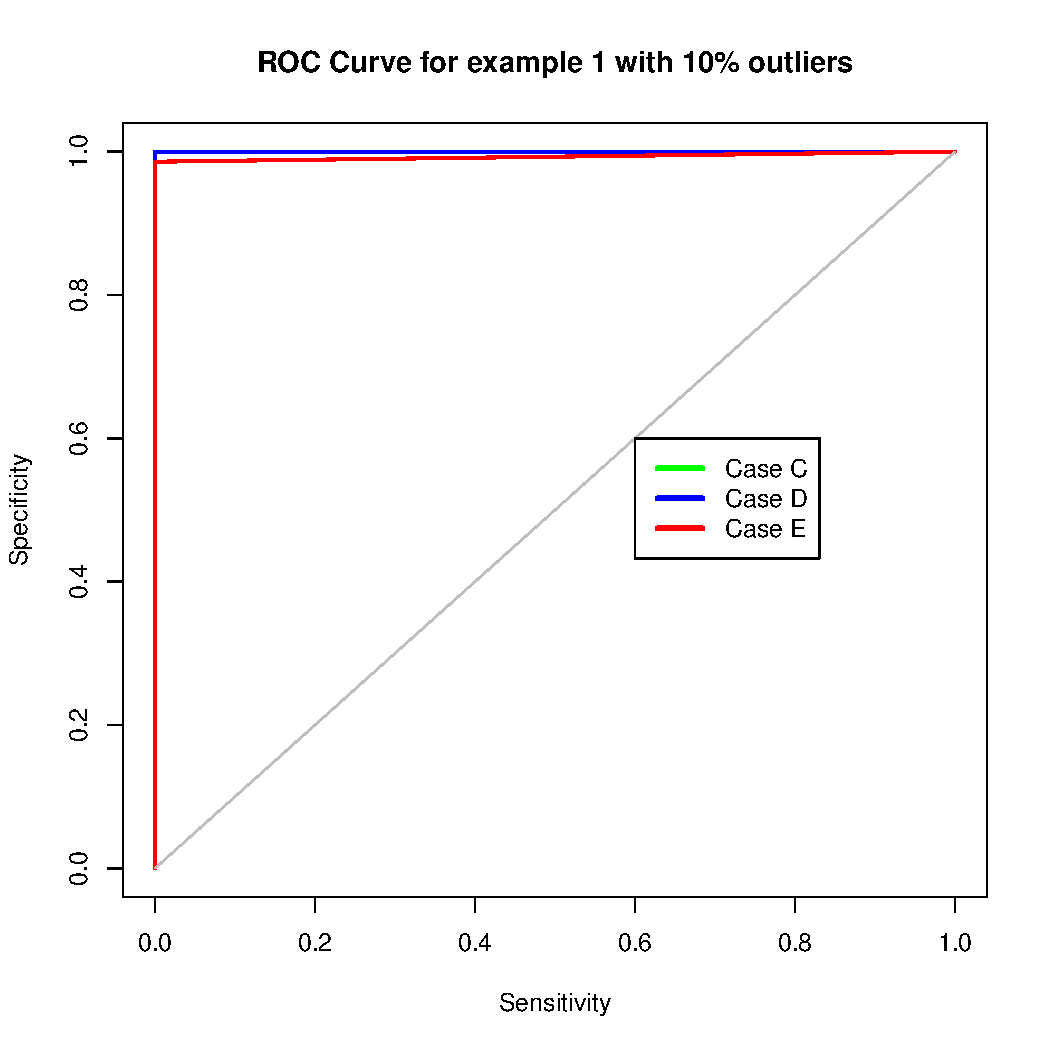
\includegraphics[width=\maxwidth]{figure/unnamed-chunk-2-1} 

\end{knitrout}
% ----------------------------- ROC Curve for example 1 with 20% outliers-------------------------------%
\begin{knitrout}
\definecolor{shadecolor}{rgb}{0.969, 0.969, 0.969}\color{fgcolor}
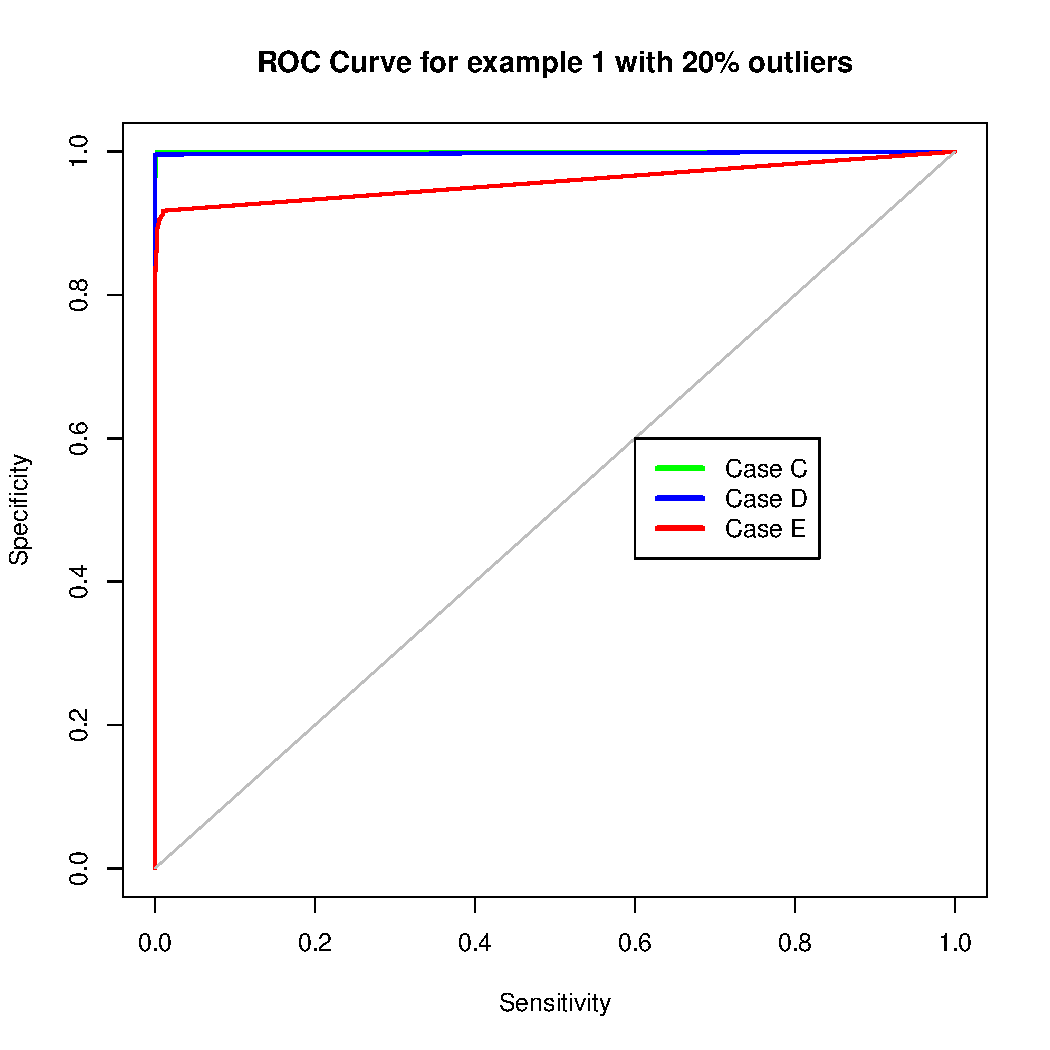
\includegraphics[width=\maxwidth]{figure/unnamed-chunk-3-1} 

\end{knitrout}
% ----------------------------- ROC Curve for example 1 with 30% outliers-------------------------------%
\begin{knitrout}
\definecolor{shadecolor}{rgb}{0.969, 0.969, 0.969}\color{fgcolor}
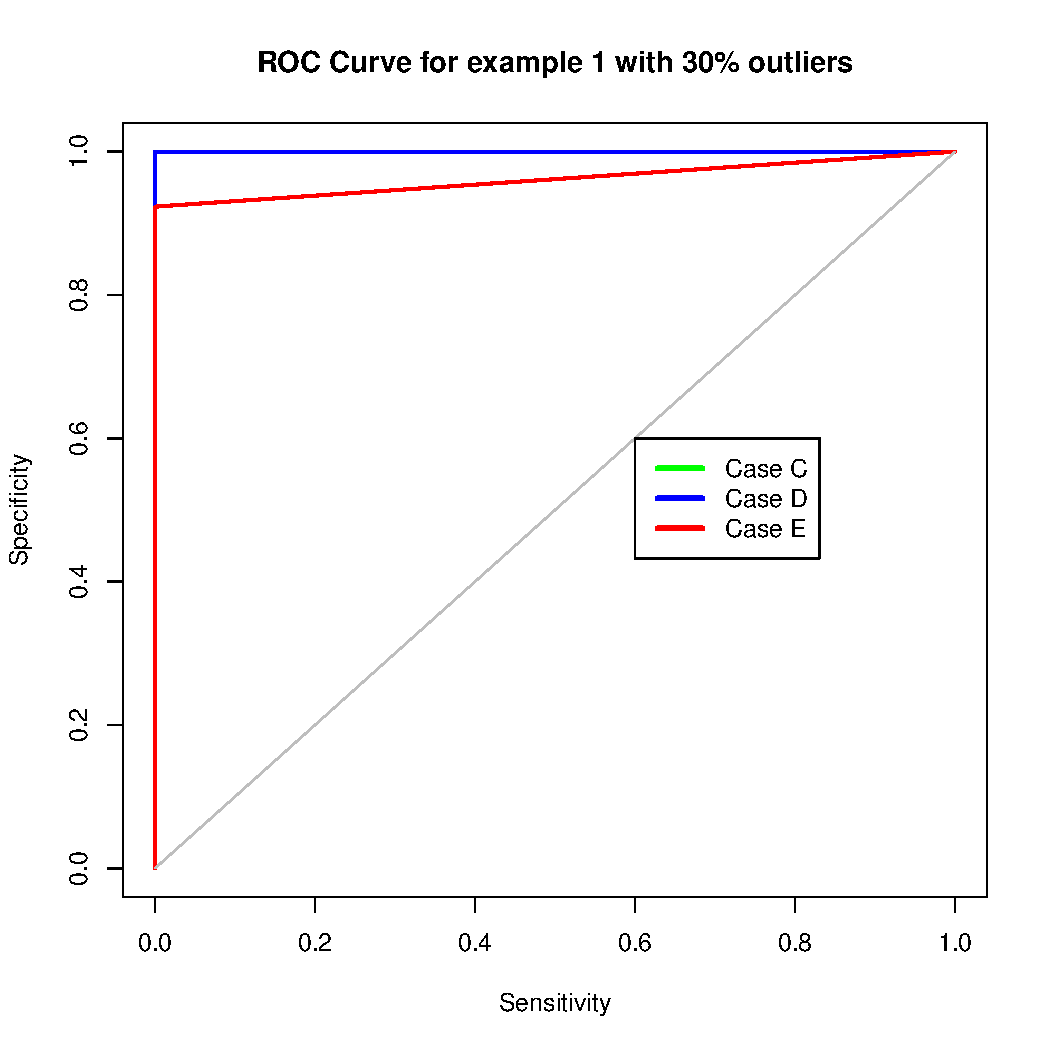
\includegraphics[width=\maxwidth]{figure/unnamed-chunk-4-1} 

\end{knitrout}

% ----------------------------- ROC Curve for example 2 with 10% outliers-------------------------------%
\begin{knitrout}
\definecolor{shadecolor}{rgb}{0.969, 0.969, 0.969}\color{fgcolor}
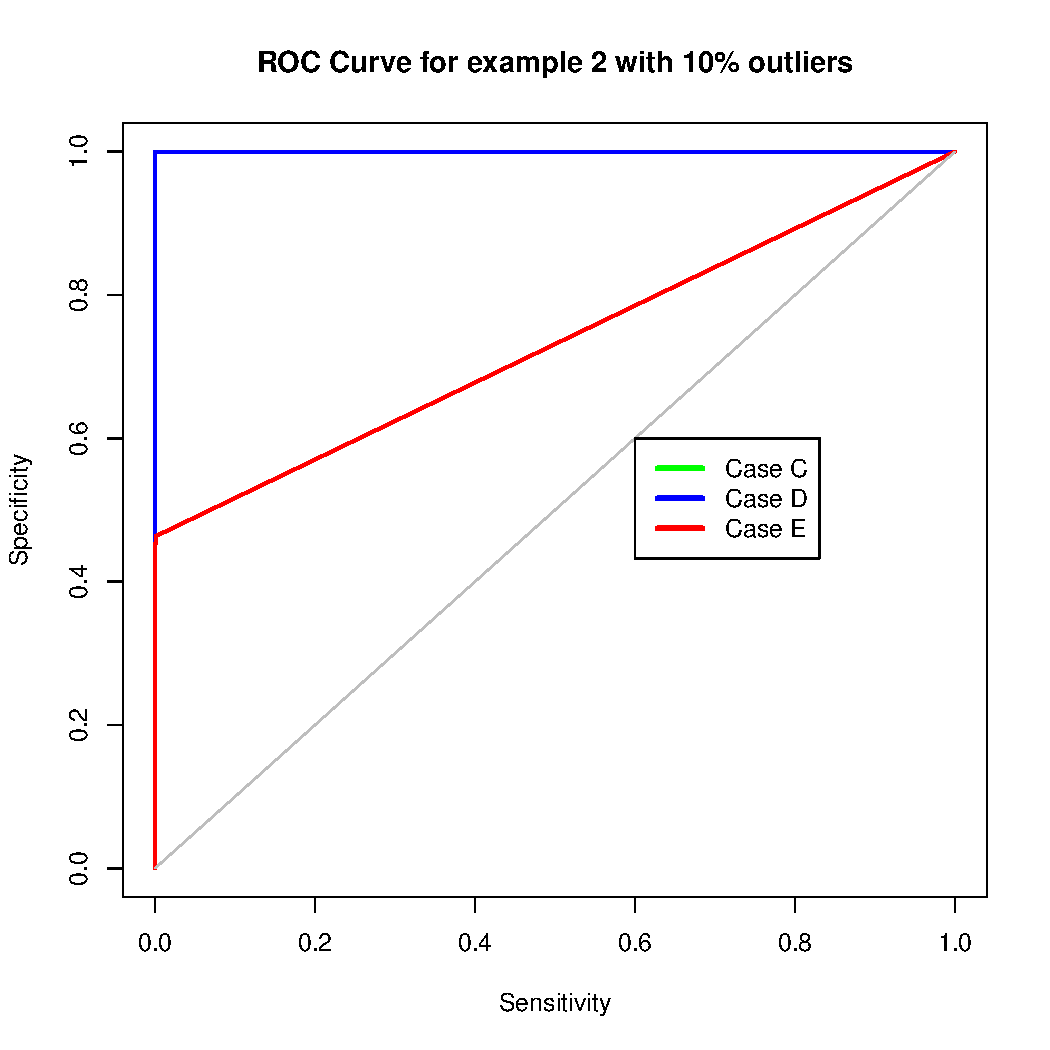
\includegraphics[width=\maxwidth]{figure/unnamed-chunk-5-1} 

\end{knitrout}

% ----------------------------- ROC Curve for example 2 with 20% outliers-------------------------------%
\begin{knitrout}
\definecolor{shadecolor}{rgb}{0.969, 0.969, 0.969}\color{fgcolor}
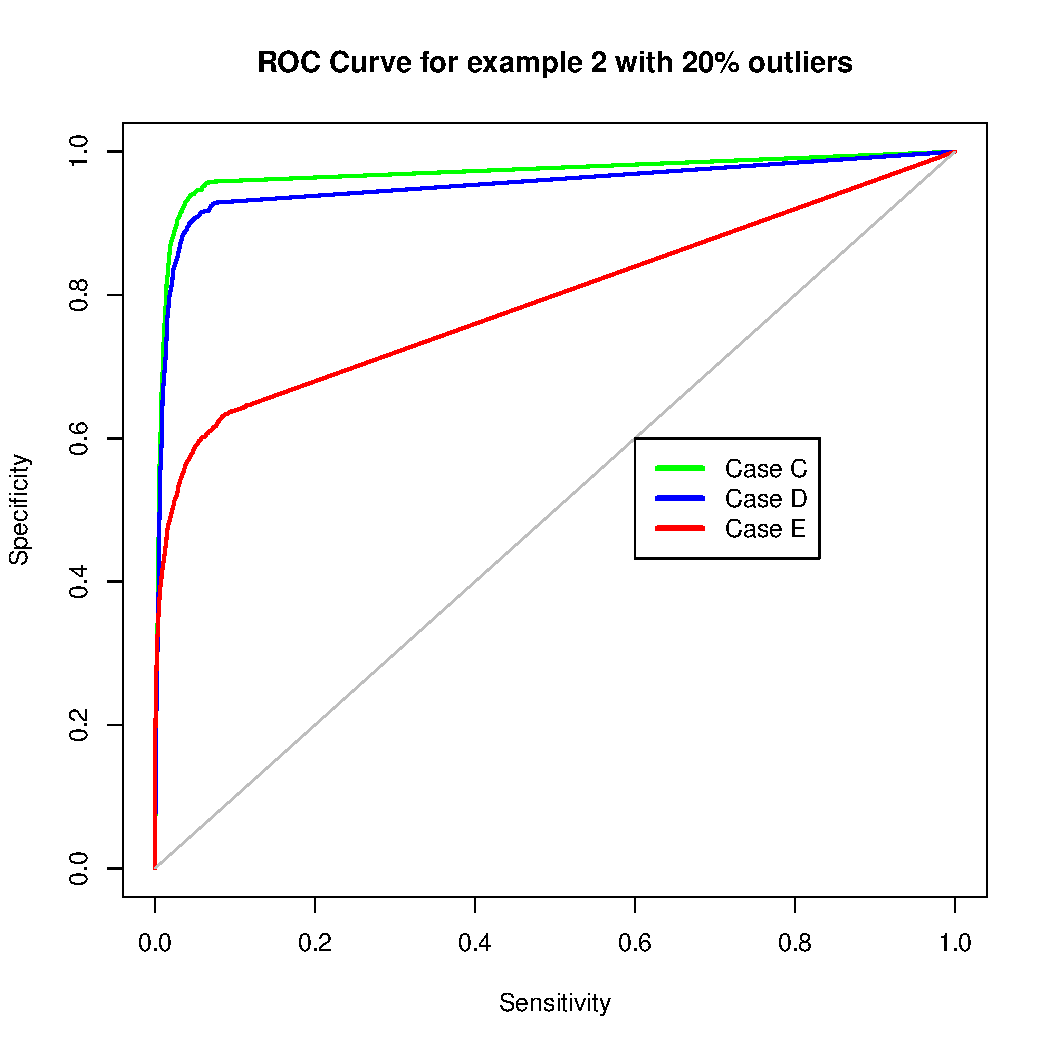
\includegraphics[width=\maxwidth]{figure/unnamed-chunk-6-1} 

\end{knitrout}

% ----------------------------- ROC Curve for example 2 with 30% outliers-------------------------------%
\begin{knitrout}
\definecolor{shadecolor}{rgb}{0.969, 0.969, 0.969}\color{fgcolor}
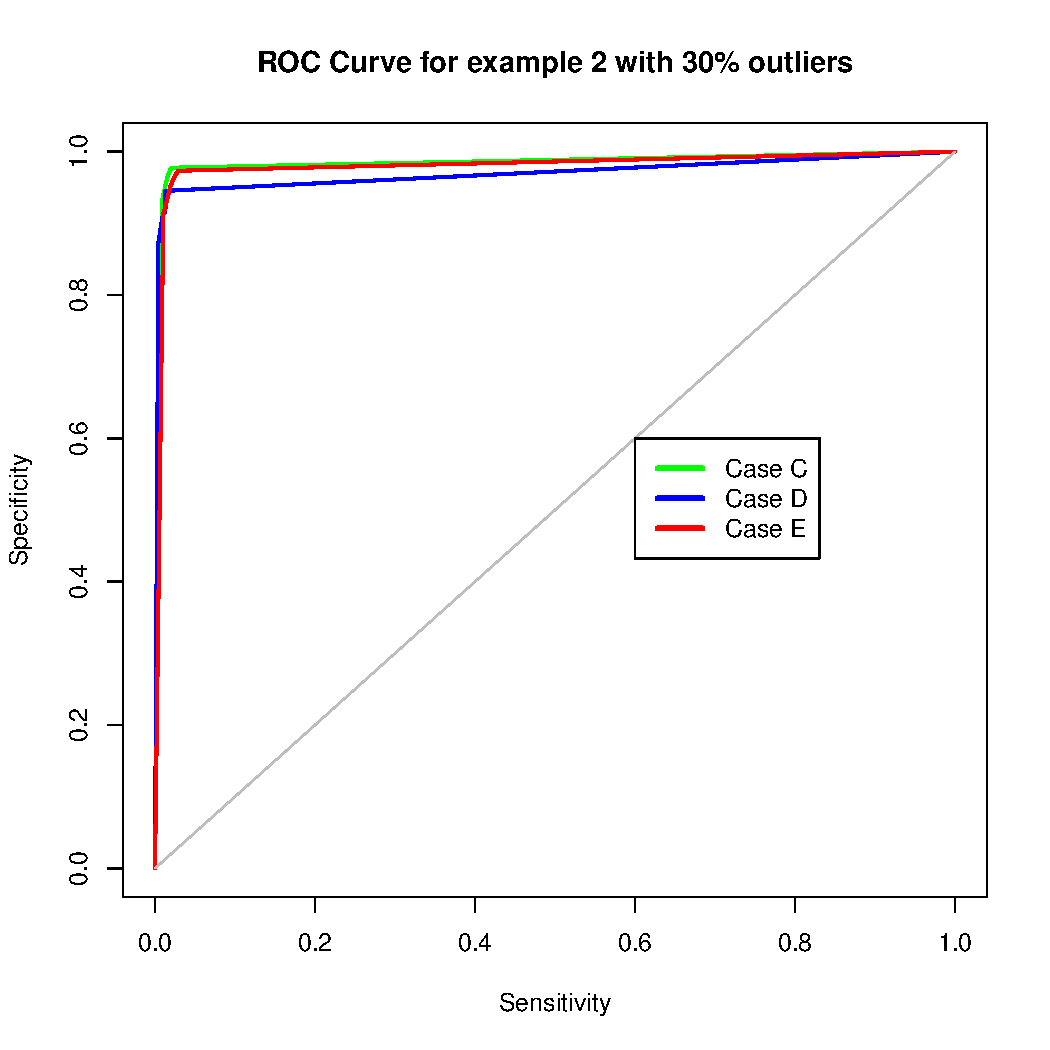
\includegraphics[width=\maxwidth]{figure/unnamed-chunk-7-1} 

\end{knitrout}
\end{document}
